\documentclass[twoside]{book}

% Packages required by doxygen
\usepackage{fixltx2e}
\usepackage{calc}
\usepackage{doxygen}
\usepackage[export]{adjustbox} % also loads graphicx
\usepackage{graphicx}
\usepackage[utf8]{inputenc}
\usepackage{makeidx}
\usepackage{multicol}
\usepackage{multirow}
\PassOptionsToPackage{warn}{textcomp}
\usepackage{textcomp}
\usepackage[nointegrals]{wasysym}
\usepackage[table]{xcolor}

% Font selection
\usepackage[T1]{fontenc}
\usepackage[scaled=.90]{helvet}
\usepackage{courier}
\usepackage{amssymb}
\usepackage{sectsty}
\renewcommand{\familydefault}{\sfdefault}
\allsectionsfont{%
  \fontseries{bc}\selectfont%
  \color{darkgray}%
}
\renewcommand{\DoxyLabelFont}{%
  \fontseries{bc}\selectfont%
  \color{darkgray}%
}
\newcommand{\+}{\discretionary{\mbox{\scriptsize$\hookleftarrow$}}{}{}}

% Page & text layout
\usepackage{geometry}
\geometry{%
  a4paper,%
  top=2.5cm,%
  bottom=2.5cm,%
  left=2.5cm,%
  right=2.5cm%
}
\tolerance=750
\hfuzz=15pt
\hbadness=750
\setlength{\emergencystretch}{15pt}
\setlength{\parindent}{0cm}
\setlength{\parskip}{3ex plus 2ex minus 2ex}
\makeatletter
\renewcommand{\paragraph}{%
  \@startsection{paragraph}{4}{0ex}{-1.0ex}{1.0ex}{%
    \normalfont\normalsize\bfseries\SS@parafont%
  }%
}
\renewcommand{\subparagraph}{%
  \@startsection{subparagraph}{5}{0ex}{-1.0ex}{1.0ex}{%
    \normalfont\normalsize\bfseries\SS@subparafont%
  }%
}
\makeatother

% Headers & footers
\usepackage{fancyhdr}
\pagestyle{fancyplain}
\fancyhead[LE]{\fancyplain{}{\bfseries\thepage}}
\fancyhead[CE]{\fancyplain{}{}}
\fancyhead[RE]{\fancyplain{}{\bfseries\leftmark}}
\fancyhead[LO]{\fancyplain{}{\bfseries\rightmark}}
\fancyhead[CO]{\fancyplain{}{}}
\fancyhead[RO]{\fancyplain{}{\bfseries\thepage}}
\fancyfoot[LE]{\fancyplain{}{}}
\fancyfoot[CE]{\fancyplain{}{}}
\fancyfoot[RE]{\fancyplain{}{\bfseries\scriptsize Generated by Doxygen }}
\fancyfoot[LO]{\fancyplain{}{\bfseries\scriptsize Generated by Doxygen }}
\fancyfoot[CO]{\fancyplain{}{}}
\fancyfoot[RO]{\fancyplain{}{}}
\renewcommand{\footrulewidth}{0.4pt}
\renewcommand{\chaptermark}[1]{%
  \markboth{#1}{}%
}
\renewcommand{\sectionmark}[1]{%
  \markright{\thesection\ #1}%
}

% Indices & bibliography
\usepackage{natbib}
\usepackage[titles]{tocloft}
\setcounter{tocdepth}{3}
\setcounter{secnumdepth}{5}
\makeindex

% Hyperlinks (required, but should be loaded last)
\usepackage{ifpdf}
\ifpdf
  \usepackage[pdftex,pagebackref=true]{hyperref}
\else
  \usepackage[ps2pdf,pagebackref=true]{hyperref}
\fi
\hypersetup{%
  colorlinks=true,%
  linkcolor=blue,%
  citecolor=blue,%
  unicode%
}

% Custom commands
\newcommand{\clearemptydoublepage}{%
  \newpage{\pagestyle{empty}\cleardoublepage}%
}

\usepackage{caption}
\captionsetup{labelsep=space,justification=centering,font={bf},singlelinecheck=off,skip=4pt,position=top}

%===== C O N T E N T S =====

\begin{document}

% Titlepage & ToC
\hypersetup{pageanchor=false,
             bookmarksnumbered=true,
             pdfencoding=unicode
            }
\pagenumbering{roman}
\begin{titlepage}
\vspace*{7cm}
\begin{center}%
{\Large lab 8 }\\
\vspace*{1cm}
{\large Generated by Doxygen 1.8.11}\\
\end{center}
\end{titlepage}
\clearemptydoublepage
\tableofcontents
\clearemptydoublepage
\pagenumbering{arabic}
\hypersetup{pageanchor=true}

%--- Begin generated contents ---
\chapter{Class Index}
\section{Class List}
Here are the classes, structs, unions and interfaces with brief descriptions\+:\begin{DoxyCompactList}
\item\contentsline{section}{\hyperlink{classParse}{Parse} \\*Defines a client request }{\pageref{classParse}}{}
\item\contentsline{section}{\hyperlink{classRepository}{Repository} \\*Defines fields of repositories }{\pageref{classRepository}}{}
\end{DoxyCompactList}

\chapter{File Index}
\section{File List}
Here is a list of all documented files with brief descriptions\+:\begin{DoxyCompactList}
\item\contentsline{section}{include/\hyperlink{https__server_8h}{https\+\_\+server.\+h} \\*Defines Server }{\pageref{https__server_8h}}{}
\item\contentsline{section}{include/\hyperlink{inputParse_8h}{input\+Parse.\+h} \\*Describes a \hyperlink{classParse}{Parse} }{\pageref{inputParse_8h}}{}
\item\contentsline{section}{include/\hyperlink{repositories_8h}{repositories.\+h} \\*General information about class \hyperlink{classRepository}{Repository} }{\pageref{repositories_8h}}{}
\item\contentsline{section}{include/\hyperlink{responce_8h}{responce.\+h} \\*Creates information about response }{\pageref{responce_8h}}{}
\end{DoxyCompactList}

\chapter{Class Documentation}
\hypertarget{classParse}{}\section{Parse Class Reference}
\label{classParse}\index{Parse@{Parse}}


defines a client request  




{\ttfamily \#include $<$input\+Parse.\+h$>$}

\subsection*{Public Member Functions}
\begin{DoxyCompactItemize}
\item 
\hyperlink{classParse_ab44bf754dbe7e6fc008af31af8ca75fb}{Parse} ()\hypertarget{classParse_ab44bf754dbe7e6fc008af31af8ca75fb}{}\label{classParse_ab44bf754dbe7e6fc008af31af8ca75fb}

\begin{DoxyCompactList}\small\item\em default public constructor for \hyperlink{classParse}{Parse} \end{DoxyCompactList}\item 
\hyperlink{classParse_aa65ad10fd2ac9eb15bf75d681e4b1d38}{Parse} (string data)
\begin{DoxyCompactList}\small\item\em public constructor for \hyperlink{classParse}{Parse} that fill all fields in \hyperlink{classParse}{Parse} \end{DoxyCompactList}\item 
string \hyperlink{classParse_afe93e93b4a3be37aa33ff811d490ea08}{get\+\_\+path} ()
\begin{DoxyCompactList}\small\item\em gets specified path from client request \end{DoxyCompactList}\item 
string \hyperlink{classParse_aaa75754008d716cf912eb0526e31ae8f}{get\+\_\+value} ()
\begin{DoxyCompactList}\small\item\em gets specified value from client request \end{DoxyCompactList}\item 
string \hyperlink{classParse_a1d8ede969d4c362b59ed7f9ff5943166}{get\+\_\+key} ()
\begin{DoxyCompactList}\small\item\em gets specified key from client request \end{DoxyCompactList}\item 
\hyperlink{classParse_a09620677a05691231960c07803aec495}{$\sim$\+Parse} ()\hypertarget{classParse_a09620677a05691231960c07803aec495}{}\label{classParse_a09620677a05691231960c07803aec495}

\begin{DoxyCompactList}\small\item\em default public destructor for \hyperlink{classParse}{Parse} \end{DoxyCompactList}\end{DoxyCompactItemize}


\subsection{Detailed Description}
defines a client request 

\subsection{Constructor \& Destructor Documentation}
\index{Parse@{Parse}!Parse@{Parse}}
\index{Parse@{Parse}!Parse@{Parse}}
\subsubsection[{\texorpdfstring{Parse(string data)}{Parse(string data)}}]{\setlength{\rightskip}{0pt plus 5cm}Parse\+::\+Parse (
\begin{DoxyParamCaption}
\item[{string}]{data}
\end{DoxyParamCaption}
)}\hypertarget{classParse_aa65ad10fd2ac9eb15bf75d681e4b1d38}{}\label{classParse_aa65ad10fd2ac9eb15bf75d681e4b1d38}


public constructor for \hyperlink{classParse}{Parse} that fill all fields in \hyperlink{classParse}{Parse} 


\begin{DoxyParams}{Parameters}
{\em string} & -\/ string that is defines client request \\
\hline
\end{DoxyParams}


\subsection{Member Function Documentation}
\index{Parse@{Parse}!get\+\_\+key@{get\+\_\+key}}
\index{get\+\_\+key@{get\+\_\+key}!Parse@{Parse}}
\subsubsection[{\texorpdfstring{get\+\_\+key()}{get_key()}}]{\setlength{\rightskip}{0pt plus 5cm}string Parse\+::get\+\_\+key (
\begin{DoxyParamCaption}
{}
\end{DoxyParamCaption}
)}\hypertarget{classParse_a1d8ede969d4c362b59ed7f9ff5943166}{}\label{classParse_a1d8ede969d4c362b59ed7f9ff5943166}


gets specified key from client request 

\begin{DoxyReturn}{Returns}
string that defines specified key 
\end{DoxyReturn}
\index{Parse@{Parse}!get\+\_\+path@{get\+\_\+path}}
\index{get\+\_\+path@{get\+\_\+path}!Parse@{Parse}}
\subsubsection[{\texorpdfstring{get\+\_\+path()}{get_path()}}]{\setlength{\rightskip}{0pt plus 5cm}string Parse\+::get\+\_\+path (
\begin{DoxyParamCaption}
{}
\end{DoxyParamCaption}
)}\hypertarget{classParse_afe93e93b4a3be37aa33ff811d490ea08}{}\label{classParse_afe93e93b4a3be37aa33ff811d490ea08}


gets specified path from client request 

\begin{DoxyReturn}{Returns}
string that defines specified path 
\end{DoxyReturn}
\index{Parse@{Parse}!get\+\_\+value@{get\+\_\+value}}
\index{get\+\_\+value@{get\+\_\+value}!Parse@{Parse}}
\subsubsection[{\texorpdfstring{get\+\_\+value()}{get_value()}}]{\setlength{\rightskip}{0pt plus 5cm}string Parse\+::get\+\_\+value (
\begin{DoxyParamCaption}
{}
\end{DoxyParamCaption}
)}\hypertarget{classParse_aaa75754008d716cf912eb0526e31ae8f}{}\label{classParse_aaa75754008d716cf912eb0526e31ae8f}


gets specified value from client request 

\begin{DoxyReturn}{Returns}
string that defines specified value 
\end{DoxyReturn}


The documentation for this class was generated from the following files\+:\begin{DoxyCompactItemize}
\item 
include/\hyperlink{inputParse_8h}{input\+Parse.\+h}\item 
src/input\+Parse.\+cpp\end{DoxyCompactItemize}

\hypertarget{classRepository}{}\section{Repository Class Reference}
\label{classRepository}\index{Repository@{Repository}}


defines fields of repositories  




{\ttfamily \#include $<$repositories.\+h$>$}

\subsection*{Public Member Functions}
\begin{DoxyCompactItemize}
\item 
\hyperlink{classRepository_acea749ed86f3239ecf20c696f721ab7e}{Repository} ()\hypertarget{classRepository_acea749ed86f3239ecf20c696f721ab7e}{}\label{classRepository_acea749ed86f3239ecf20c696f721ab7e}

\begin{DoxyCompactList}\small\item\em default public constructor for \hyperlink{classRepository}{Repository} \end{DoxyCompactList}\item 
\hyperlink{classRepository_ae706286558286f91aecf1274c0e730ea}{Repository} (int \hyperlink{classRepository_a939747771b843e2e6ac651bdf273ec0f}{id}, std\+::string \hyperlink{classRepository_a8d967c3615e5a68be145889fb23aac14}{name}, std\+::string \hyperlink{classRepository_adffe93ad41af4c08c3adb8bcb1ea12fa}{language}, std\+::string \hyperlink{classRepository_a81933778a20e63810589ebc9de593782}{description})
\begin{DoxyCompactList}\small\item\em public constructor for \hyperlink{classRepository}{Repository} that fill all fields in \hyperlink{classRepository}{Repository} \end{DoxyCompactList}\item 
\hyperlink{classRepository_a26ba073b495c4b231658713f1e3ffeae}{$\sim$\+Repository} ()\hypertarget{classRepository_a26ba073b495c4b231658713f1e3ffeae}{}\label{classRepository_a26ba073b495c4b231658713f1e3ffeae}

\begin{DoxyCompactList}\small\item\em default public destructor for \hyperlink{classRepository}{Repository} \end{DoxyCompactList}\item 
void \hyperlink{classRepository_a41e85c3ea1a98682066fca0d9386dd72}{set\+\_\+name} (std\+::string \hyperlink{classRepository_a8d967c3615e5a68be145889fb23aac14}{name})
\begin{DoxyCompactList}\small\item\em sets name of repository \end{DoxyCompactList}\item 
void \hyperlink{classRepository_a42c5546e4289a197a5dc5b57e3b20c73}{set\+\_\+language} (std\+::string \hyperlink{classRepository_adffe93ad41af4c08c3adb8bcb1ea12fa}{language})
\begin{DoxyCompactList}\small\item\em sets programming language of repository \end{DoxyCompactList}\item 
void \hyperlink{classRepository_a6db26d595479cb9bad8f77c71cace7f0}{set\+\_\+description} (std\+::string \hyperlink{classRepository_a81933778a20e63810589ebc9de593782}{description})
\begin{DoxyCompactList}\small\item\em sets general information about repository \end{DoxyCompactList}\item 
void \hyperlink{classRepository_a55158dd3fae6d0baaff29557c4a853b4}{set\+\_\+id} (int \hyperlink{classRepository_a939747771b843e2e6ac651bdf273ec0f}{id})
\begin{DoxyCompactList}\small\item\em sets unique id of repository \end{DoxyCompactList}\item 
std\+::string \hyperlink{classRepository_a8d967c3615e5a68be145889fb23aac14}{name} ()
\begin{DoxyCompactList}\small\item\em get name of repository \end{DoxyCompactList}\item 
std\+::string \hyperlink{classRepository_adffe93ad41af4c08c3adb8bcb1ea12fa}{language} ()
\begin{DoxyCompactList}\small\item\em get programming language of repository \end{DoxyCompactList}\item 
int \hyperlink{classRepository_a939747771b843e2e6ac651bdf273ec0f}{id} ()
\begin{DoxyCompactList}\small\item\em get id of repository \end{DoxyCompactList}\item 
std\+::string \hyperlink{classRepository_a81933778a20e63810589ebc9de593782}{description} ()
\begin{DoxyCompactList}\small\item\em get description of repository \end{DoxyCompactList}\item 
void \hyperlink{classRepository_a2ecd8cabd6d37be033d3f4bf8e90f5ae}{print} ()
\end{DoxyCompactItemize}


\subsection{Detailed Description}
defines fields of repositories 

\subsection{Constructor \& Destructor Documentation}
\index{Repository@{Repository}!Repository@{Repository}}
\index{Repository@{Repository}!Repository@{Repository}}
\subsubsection[{\texorpdfstring{Repository(int id, std\+::string name, std\+::string language, std\+::string description)}{Repository(int id, std::string name, std::string language, std::string description)}}]{\setlength{\rightskip}{0pt plus 5cm}Repository\+::\+Repository (
\begin{DoxyParamCaption}
\item[{int}]{id, }
\item[{std\+::string}]{name, }
\item[{std\+::string}]{language, }
\item[{std\+::string}]{description}
\end{DoxyParamCaption}
)}\hypertarget{classRepository_ae706286558286f91aecf1274c0e730ea}{}\label{classRepository_ae706286558286f91aecf1274c0e730ea}


public constructor for \hyperlink{classRepository}{Repository} that fill all fields in \hyperlink{classRepository}{Repository} 


\begin{DoxyParams}{Parameters}
{\em id} & -\/ unique key of repository \\
\hline
{\em name} & -\/ name of repository \\
\hline
{\em language} & -\/ a programming language \\
\hline
{\em description} & -\/ general information about repository \\
\hline
\end{DoxyParams}


\subsection{Member Function Documentation}
\index{Repository@{Repository}!description@{description}}
\index{description@{description}!Repository@{Repository}}
\subsubsection[{\texorpdfstring{description()}{description()}}]{\setlength{\rightskip}{0pt plus 5cm}std\+::string Repository\+::description (
\begin{DoxyParamCaption}
{}
\end{DoxyParamCaption}
)}\hypertarget{classRepository_a81933778a20e63810589ebc9de593782}{}\label{classRepository_a81933778a20e63810589ebc9de593782}


get description of repository 

\begin{DoxyReturn}{Returns}
string that represents description of repository 
\end{DoxyReturn}
\index{Repository@{Repository}!id@{id}}
\index{id@{id}!Repository@{Repository}}
\subsubsection[{\texorpdfstring{id()}{id()}}]{\setlength{\rightskip}{0pt plus 5cm}int Repository\+::id (
\begin{DoxyParamCaption}
{}
\end{DoxyParamCaption}
)}\hypertarget{classRepository_a939747771b843e2e6ac651bdf273ec0f}{}\label{classRepository_a939747771b843e2e6ac651bdf273ec0f}


get id of repository 

\begin{DoxyReturn}{Returns}
string that represents id of repository 
\end{DoxyReturn}
\index{Repository@{Repository}!language@{language}}
\index{language@{language}!Repository@{Repository}}
\subsubsection[{\texorpdfstring{language()}{language()}}]{\setlength{\rightskip}{0pt plus 5cm}std\+::string Repository\+::language (
\begin{DoxyParamCaption}
{}
\end{DoxyParamCaption}
)}\hypertarget{classRepository_adffe93ad41af4c08c3adb8bcb1ea12fa}{}\label{classRepository_adffe93ad41af4c08c3adb8bcb1ea12fa}


get programming language of repository 

\begin{DoxyReturn}{Returns}
string that represents programming language of repository 
\end{DoxyReturn}
\index{Repository@{Repository}!name@{name}}
\index{name@{name}!Repository@{Repository}}
\subsubsection[{\texorpdfstring{name()}{name()}}]{\setlength{\rightskip}{0pt plus 5cm}std\+::string Repository\+::name (
\begin{DoxyParamCaption}
{}
\end{DoxyParamCaption}
)}\hypertarget{classRepository_a8d967c3615e5a68be145889fb23aac14}{}\label{classRepository_a8d967c3615e5a68be145889fb23aac14}


get name of repository 

\begin{DoxyReturn}{Returns}
string that represents name of repository 
\end{DoxyReturn}
\index{Repository@{Repository}!print@{print}}
\index{print@{print}!Repository@{Repository}}
\subsubsection[{\texorpdfstring{print()}{print()}}]{\setlength{\rightskip}{0pt plus 5cm}void Repository\+::print (
\begin{DoxyParamCaption}
{}
\end{DoxyParamCaption}
)}\hypertarget{classRepository_a2ecd8cabd6d37be033d3f4bf8e90f5ae}{}\label{classRepository_a2ecd8cabd6d37be033d3f4bf8e90f5ae}
data to the screen \index{Repository@{Repository}!set\+\_\+description@{set\+\_\+description}}
\index{set\+\_\+description@{set\+\_\+description}!Repository@{Repository}}
\subsubsection[{\texorpdfstring{set\+\_\+description(std\+::string description)}{set_description(std::string description)}}]{\setlength{\rightskip}{0pt plus 5cm}void Repository\+::set\+\_\+description (
\begin{DoxyParamCaption}
\item[{std\+::string}]{description}
\end{DoxyParamCaption}
)}\hypertarget{classRepository_a6db26d595479cb9bad8f77c71cace7f0}{}\label{classRepository_a6db26d595479cb9bad8f77c71cace7f0}


sets general information about repository 


\begin{DoxyParams}{Parameters}
{\em description} & -\/ description of repository \\
\hline
\end{DoxyParams}
\index{Repository@{Repository}!set\+\_\+id@{set\+\_\+id}}
\index{set\+\_\+id@{set\+\_\+id}!Repository@{Repository}}
\subsubsection[{\texorpdfstring{set\+\_\+id(int id)}{set_id(int id)}}]{\setlength{\rightskip}{0pt plus 5cm}void Repository\+::set\+\_\+id (
\begin{DoxyParamCaption}
\item[{int}]{id}
\end{DoxyParamCaption}
)}\hypertarget{classRepository_a55158dd3fae6d0baaff29557c4a853b4}{}\label{classRepository_a55158dd3fae6d0baaff29557c4a853b4}


sets unique id of repository 


\begin{DoxyParams}{Parameters}
{\em id} & -\/ unique key \\
\hline
\end{DoxyParams}
\index{Repository@{Repository}!set\+\_\+language@{set\+\_\+language}}
\index{set\+\_\+language@{set\+\_\+language}!Repository@{Repository}}
\subsubsection[{\texorpdfstring{set\+\_\+language(std\+::string language)}{set_language(std::string language)}}]{\setlength{\rightskip}{0pt plus 5cm}void Repository\+::set\+\_\+language (
\begin{DoxyParamCaption}
\item[{std\+::string}]{language}
\end{DoxyParamCaption}
)}\hypertarget{classRepository_a42c5546e4289a197a5dc5b57e3b20c73}{}\label{classRepository_a42c5546e4289a197a5dc5b57e3b20c73}


sets programming language of repository 


\begin{DoxyParams}{Parameters}
{\em language} & -\/ programming language of repository \\
\hline
\end{DoxyParams}
\index{Repository@{Repository}!set\+\_\+name@{set\+\_\+name}}
\index{set\+\_\+name@{set\+\_\+name}!Repository@{Repository}}
\subsubsection[{\texorpdfstring{set\+\_\+name(std\+::string name)}{set_name(std::string name)}}]{\setlength{\rightskip}{0pt plus 5cm}void Repository\+::set\+\_\+name (
\begin{DoxyParamCaption}
\item[{std\+::string}]{name}
\end{DoxyParamCaption}
)}\hypertarget{classRepository_a41e85c3ea1a98682066fca0d9386dd72}{}\label{classRepository_a41e85c3ea1a98682066fca0d9386dd72}


sets name of repository 


\begin{DoxyParams}{Parameters}
{\em name} & -\/ name of repository \\
\hline
\end{DoxyParams}


The documentation for this class was generated from the following files\+:\begin{DoxyCompactItemize}
\item 
include/\hyperlink{repositories_8h}{repositories.\+h}\item 
src/repositories.\+cpp\end{DoxyCompactItemize}

\chapter{File Documentation}
\hypertarget{https__server_8h}{}\section{include/https\+\_\+server.h File Reference}
\label{https__server_8h}\index{include/https\+\_\+server.\+h@{include/https\+\_\+server.\+h}}


defines Server  


{\ttfamily \#include $<$iostream$>$}\\*
Include dependency graph for https\+\_\+server.\+h\+:
\nopagebreak
\begin{figure}[H]
\begin{center}
\leavevmode
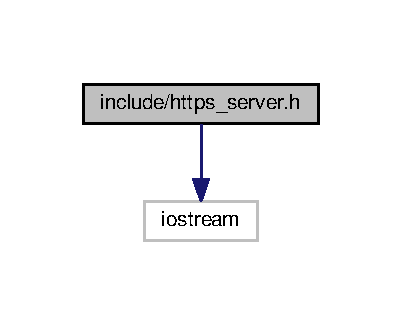
\includegraphics[width=193pt]{https__server_8h__incl}
\end{center}
\end{figure}
\subsection*{Functions}
\begin{DoxyCompactItemize}
\item 
int \hyperlink{https__server_8h_aa8b391a3236cabb4afbc1ed866a9ef2e}{http\+\_\+server} ()\hypertarget{https__server_8h_aa8b391a3236cabb4afbc1ed866a9ef2e}{}\label{https__server_8h_aa8b391a3236cabb4afbc1ed866a9ef2e}

\begin{DoxyCompactList}\small\item\em 
\begin{DoxyItemize}
\item H\+T\+TP server 
\end{DoxyItemize}\end{DoxyCompactList}\end{DoxyCompactItemize}


\subsection{Detailed Description}
defines Server 


\hypertarget{inputParse_8h}{}\section{include/input\+Parse.h File Reference}
\label{inputParse_8h}\index{include/input\+Parse.\+h@{include/input\+Parse.\+h}}


describes a \hyperlink{classParse}{Parse}  


{\ttfamily \#include $<$iostream$>$}\\*
Include dependency graph for input\+Parse.\+h\+:
\nopagebreak
\begin{figure}[H]
\begin{center}
\leavevmode
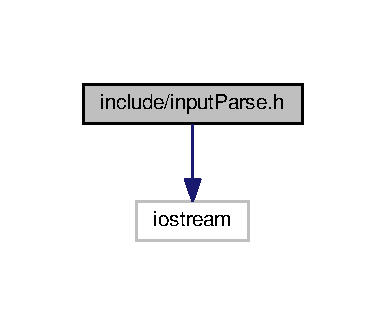
\includegraphics[width=185pt]{inputParse_8h__incl}
\end{center}
\end{figure}
\subsection*{Classes}
\begin{DoxyCompactItemize}
\item 
class \hyperlink{classParse}{Parse}
\begin{DoxyCompactList}\small\item\em defines a client request \end{DoxyCompactList}\end{DoxyCompactItemize}


\subsection{Detailed Description}
describes a \hyperlink{classParse}{Parse} 


\hypertarget{repositories_8h}{}\section{include/repositories.h File Reference}
\label{repositories_8h}\index{include/repositories.\+h@{include/repositories.\+h}}


general information about class \hyperlink{classRepository}{Repository}  


{\ttfamily \#include $<$iostream$>$}\\*
Include dependency graph for repositories.\+h\+:
\nopagebreak
\begin{figure}[H]
\begin{center}
\leavevmode
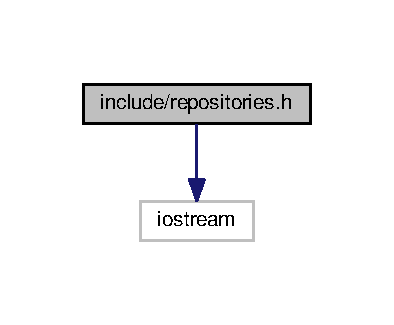
\includegraphics[width=189pt]{repositories_8h__incl}
\end{center}
\end{figure}
This graph shows which files directly or indirectly include this file\+:
\nopagebreak
\begin{figure}[H]
\begin{center}
\leavevmode
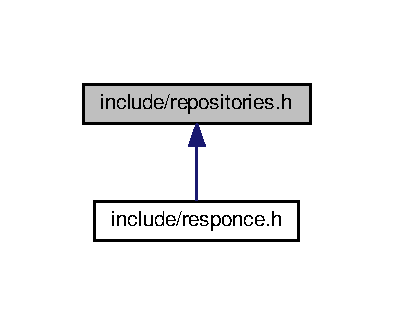
\includegraphics[width=189pt]{repositories_8h__dep__incl}
\end{center}
\end{figure}
\subsection*{Classes}
\begin{DoxyCompactItemize}
\item 
class \hyperlink{classRepository}{Repository}
\begin{DoxyCompactList}\small\item\em defines fields of repositories \end{DoxyCompactList}\end{DoxyCompactItemize}


\subsection{Detailed Description}
general information about class \hyperlink{classRepository}{Repository} 


\hypertarget{responce_8h}{}\section{include/responce.h File Reference}
\label{responce_8h}\index{include/responce.\+h@{include/responce.\+h}}


creates information about response  


{\ttfamily \#include $<$iostream$>$}\\*
{\ttfamily \#include $<$string$>$}\\*
{\ttfamily \#include $<$vector$>$}\\*
{\ttfamily \#include \char`\"{}repositories.\+h\char`\"{}}\\*
Include dependency graph for responce.\+h\+:
\nopagebreak
\begin{figure}[H]
\begin{center}
\leavevmode
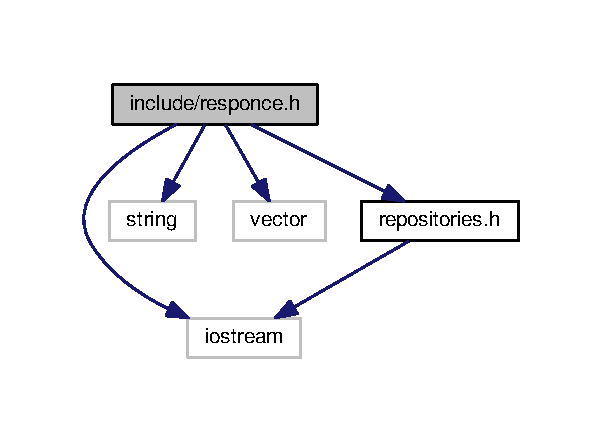
\includegraphics[width=289pt]{responce_8h__incl}
\end{center}
\end{figure}
\subsection*{Functions}
\begin{DoxyCompactItemize}
\item 
string \hyperlink{responce_8h_af84f671a64834cb5121503d634eb3543}{information\+\_\+about\+\_\+server} ()
\begin{DoxyCompactList}\small\item\em creates information about server \end{DoxyCompactList}\item 
string \hyperlink{responce_8h_a7d847248c61ad8e413d98ac718733964}{Favourite\+Repository} (vector$<$ \hyperlink{classRepository}{Repository} $\ast$ $>$ repository)
\begin{DoxyCompactList}\small\item\em creates information about favorite repositories \end{DoxyCompactList}\item 
string \hyperlink{responce_8h_aefadbf51dcf80da5005c397a84896be2}{find\+Where\+Id\+Is} (vector$<$ \hyperlink{classRepository}{Repository} $\ast$ $>$ repository, string data\+As\+String, string key)
\begin{DoxyCompactList}\small\item\em creates information about some repositories, by field id \end{DoxyCompactList}\item 
string \hyperlink{responce_8h_a835c5691f8e6512057a87e86169a0164}{get\+File} ()
\begin{DoxyCompactList}\small\item\em creates information about file \char`\"{}data.\+txt\char`\"{} \end{DoxyCompactList}\item 
string \hyperlink{responce_8h_ae60f8e88a80a035785b1a5c8dc438b4d}{find\+Key\+Value} (vector$<$ \hyperlink{classRepository}{Repository} $\ast$ $>$ repository, string data\+As\+String, string key)
\begin{DoxyCompactList}\small\item\em creates information about some repositories, by field key = value \end{DoxyCompactList}\item 
string \hyperlink{responce_8h_abbf7ee804ee2e9a9ed56d23212a201a6}{get\+File\+Letter} ()
\begin{DoxyCompactList}\small\item\em creates information about letters in file \char`\"{}data.\+txt\char`\"{} \end{DoxyCompactList}\end{DoxyCompactItemize}


\subsection{Detailed Description}
creates information about response 



\subsection{Function Documentation}
\index{responce.\+h@{responce.\+h}!Favourite\+Repository@{Favourite\+Repository}}
\index{Favourite\+Repository@{Favourite\+Repository}!responce.\+h@{responce.\+h}}
\subsubsection[{\texorpdfstring{Favourite\+Repository(vector$<$ Repository $\ast$ $>$ repository)}{FavouriteRepository(vector< Repository * > repository)}}]{\setlength{\rightskip}{0pt plus 5cm}string Favourite\+Repository (
\begin{DoxyParamCaption}
\item[{vector$<$ {\bf Repository} $\ast$ $>$}]{repository}
\end{DoxyParamCaption}
)}\hypertarget{responce_8h_a7d847248c61ad8e413d98ac718733964}{}\label{responce_8h_a7d847248c61ad8e413d98ac718733964}


creates information about favorite repositories 


\begin{DoxyParams}{Parameters}
{\em repository} & -\/ my favorite repositories \\
\hline
\end{DoxyParams}
\begin{DoxyReturn}{Returns}
response on \char`\"{}/favorites\char`\"{} 
\end{DoxyReturn}
\index{responce.\+h@{responce.\+h}!find\+Key\+Value@{find\+Key\+Value}}
\index{find\+Key\+Value@{find\+Key\+Value}!responce.\+h@{responce.\+h}}
\subsubsection[{\texorpdfstring{find\+Key\+Value(vector$<$ Repository $\ast$ $>$ repository, string data\+As\+String, string key)}{findKeyValue(vector< Repository * > repository, string dataAsString, string key)}}]{\setlength{\rightskip}{0pt plus 5cm}string find\+Key\+Value (
\begin{DoxyParamCaption}
\item[{vector$<$ {\bf Repository} $\ast$ $>$}]{repository, }
\item[{string}]{data\+As\+String, }
\item[{string}]{key}
\end{DoxyParamCaption}
)}\hypertarget{responce_8h_ae60f8e88a80a035785b1a5c8dc438b4d}{}\label{responce_8h_ae60f8e88a80a035785b1a5c8dc438b4d}


creates information about some repositories, by field key = value 


\begin{DoxyParams}{Parameters}
{\em repository} & -\/ my favorite repositories \\
\hline
{\em data\+As\+String} & -\/ input string \\
\hline
{\em key} & name of field \\
\hline
\end{DoxyParams}
\begin{DoxyReturn}{Returns}
response on \char`\"{}/favorites?somefield=value\char`\"{} 
\end{DoxyReturn}
\index{responce.\+h@{responce.\+h}!find\+Where\+Id\+Is@{find\+Where\+Id\+Is}}
\index{find\+Where\+Id\+Is@{find\+Where\+Id\+Is}!responce.\+h@{responce.\+h}}
\subsubsection[{\texorpdfstring{find\+Where\+Id\+Is(vector$<$ Repository $\ast$ $>$ repository, string data\+As\+String, string key)}{findWhereIdIs(vector< Repository * > repository, string dataAsString, string key)}}]{\setlength{\rightskip}{0pt plus 5cm}string find\+Where\+Id\+Is (
\begin{DoxyParamCaption}
\item[{vector$<$ {\bf Repository} $\ast$ $>$}]{repository, }
\item[{string}]{data\+As\+String, }
\item[{string}]{key}
\end{DoxyParamCaption}
)}\hypertarget{responce_8h_aefadbf51dcf80da5005c397a84896be2}{}\label{responce_8h_aefadbf51dcf80da5005c397a84896be2}


creates information about some repositories, by field id 


\begin{DoxyParams}{Parameters}
{\em repository} & -\/ my favorite repositories \\
\hline
{\em data\+As\+String} & -\/ input string \\
\hline
{\em key} & name of field \\
\hline
\end{DoxyParams}
\begin{DoxyReturn}{Returns}
response on \char`\"{}/favorites/\char`\"{} 
\end{DoxyReturn}
\index{responce.\+h@{responce.\+h}!get\+File@{get\+File}}
\index{get\+File@{get\+File}!responce.\+h@{responce.\+h}}
\subsubsection[{\texorpdfstring{get\+File()}{getFile()}}]{\setlength{\rightskip}{0pt plus 5cm}string get\+File (
\begin{DoxyParamCaption}
{}
\end{DoxyParamCaption}
)}\hypertarget{responce_8h_a835c5691f8e6512057a87e86169a0164}{}\label{responce_8h_a835c5691f8e6512057a87e86169a0164}


creates information about file \char`\"{}data.\+txt\char`\"{} 

\begin{DoxyReturn}{Returns}
response to \char`\"{}/file\char`\"{} 
\end{DoxyReturn}
\index{responce.\+h@{responce.\+h}!get\+File\+Letter@{get\+File\+Letter}}
\index{get\+File\+Letter@{get\+File\+Letter}!responce.\+h@{responce.\+h}}
\subsubsection[{\texorpdfstring{get\+File\+Letter()}{getFileLetter()}}]{\setlength{\rightskip}{0pt plus 5cm}string get\+File\+Letter (
\begin{DoxyParamCaption}
{}
\end{DoxyParamCaption}
)}\hypertarget{responce_8h_abbf7ee804ee2e9a9ed56d23212a201a6}{}\label{responce_8h_abbf7ee804ee2e9a9ed56d23212a201a6}


creates information about letters in file \char`\"{}data.\+txt\char`\"{} 

\begin{DoxyReturn}{Returns}
response to \char`\"{}/file/data\char`\"{} 
\end{DoxyReturn}
\index{responce.\+h@{responce.\+h}!information\+\_\+about\+\_\+server@{information\+\_\+about\+\_\+server}}
\index{information\+\_\+about\+\_\+server@{information\+\_\+about\+\_\+server}!responce.\+h@{responce.\+h}}
\subsubsection[{\texorpdfstring{information\+\_\+about\+\_\+server()}{information_about_server()}}]{\setlength{\rightskip}{0pt plus 5cm}string information\+\_\+about\+\_\+server (
\begin{DoxyParamCaption}
{}
\end{DoxyParamCaption}
)}\hypertarget{responce_8h_af84f671a64834cb5121503d634eb3543}{}\label{responce_8h_af84f671a64834cb5121503d634eb3543}


creates information about server 

\begin{DoxyReturn}{Returns}
response to \char`\"{}/\char`\"{} 
\end{DoxyReturn}

%--- End generated contents ---

% Index
\backmatter
\newpage
\phantomsection
\clearemptydoublepage
\addcontentsline{toc}{chapter}{Index}
\printindex

\end{document}
